%%%%%%%%%%%%%%%%%%%%%%%%%%%%%%%%%%%%%%%%%%%%%%%%%%%%%%%%%%%%%%%%%%%%%%%
%%%%%%%%%%%%%%%%%%%%%%%%%%%%%%%%%%%%%%%%%%%%%%%%%%%%%%%%%%%%%%%%%%%%%%%
%%%%%                                                                 %
%%%%%     <file_name>.tex                                             %
%%%%%                                                                 %
%%%%% Author:      <author>                                           %
%%%%% Created:     <date>                                             %
%%%%% Description: <description>                                      %
%%%%%                                                                 %
%%%%%%%%%%%%%%%%%%%%%%%%%%%%%%%%%%%%%%%%%%%%%%%%%%%%%%%%%%%%%%%%%%%%%%%
%%%%%%%%%%%%%%%%%%%%%%%%%%%%%%%%%%%%%%%%%%%%%%%%%%%%%%%%%%%%%%%%%%%%%%%

\chapter{Introduction}

Microprocessors for Internet of Things devices, wearables, smartphones, sensors and
medical devices have to work in very energy constrained environments while at
the same time providing a high amount of processing power.
Energy efficiency is thus essential for those kind of devices.
The energy needed for a certain application is the product of the power needed
during its execution and the time required to execute it.

Power consumption can be reduced by operating the digital circuit at the most
energy efficient operating point. This operating point lies near the threshold
voltage of the technology at hand \cite{NTC} as dynamic power scales
quadratically with the supply voltage. Lowering the supply voltage to
near-threshold values leads to an inevitable increase in leakage which
eventually dominates the energy consumption of the circuit, see
Figure~\ref{fig:dyn_leakage} for an example on a 32nm technology \cite{VIVEK}.
One thus has to balance between dynamic energy and leakage. At this operating
point the circuit will only achieve a low frequency compared to higher supply
voltages, which means that the performance will decrease and thus the time that
the circuit needs to be active gets longer. To reduce the active time while not
increasing the power consumption overproportionally, multiple cores can be used
that share the common infrastructure like instruction caches, scratchpad memory
and peripherals. Since the performance of the core has a direct impact on the
time our circuit needs to be active, increasing it can lead to a higher energy
efficiency of the whole system.

\begin{figure}[H]
  \centering 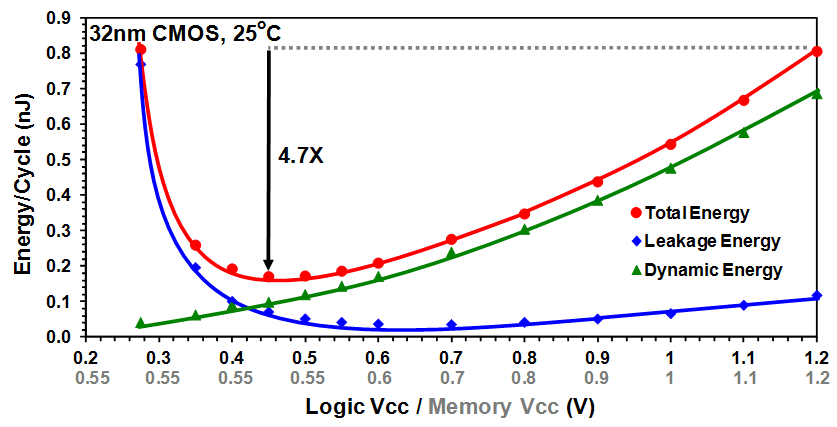
\includegraphics[width=0.7\textwidth]{./figures/dyn_leakage}
  \caption{Dynamic vs. leakage energy.}
  \label{fig:dyn_leakage}
\end{figure}

It is the goal of this thesis to increase the energy efficiency and performance
of the \orion core by adding specialized instructions. Those instructions allow
to perform more computations per clock cycle and thus the core needs less time
to process its workload.
Our goal was to add instructions to the OpenRISC \gls{ISA} that add little
overhead in terms of area and pipeline stage delay and thus have little impact
on the energy efficiency and performance when those new instructions are not
used. Since we are working on a many-core cluster platform, it was important
that our changes also work well in this cluster environment. Our focus lay on
adding vectorial support to exploit sub-word parallelism and multiplier
improvements to make the commonly used multiplication operations as fast as
possible. Together with previous \gls{ISA} extensions we achieved a speedup of
up to 5x when using those extensions. Additionally we added bit counting
instructions which can speed up some specific applications up to 35x.

Since this OpenRISC core is used in many projects that are produced as
\glspl{ASIC}, we also wanted to add some features that are usually present in
modern \glspl{CPU}. For example we have added interrupt support and in-circuit
debugging facilities.

This report is structured as follows. In Chapter~\ref{chapter:background} 
background about the platform which was used for this thesis is given.
In Chapter~\ref{chapter:related_work} an overview over related work is
presented.
In Chapter~\ref{chapter:vectorial} the changes to the \gls{ISA} are explained
and  implementation details are given, while the encoding and semantics of
the new instructions are available in Appendix~\ref{chap:instr_encoding}.
In Chapter~\ref{chapter:debug} the debug facilities that were added to the core
are described.
Chapter~\ref{chapter:changes} highlights the microarchitectural changes that
were performed.
In Chapter~\ref{chapter:results} we compare our results of the improved \orion
core with the industry standard ARM Cortex M4 and the old OR1200 OpenRISC core.
Finally Chapter~\ref{chapter:conclusion} draws a conclusion over the changes
that were done to the core during this thesis while
Chapter~\ref{chapter:outlook} gives an outlook over future work.



%%% Local Variables: 
%%% mode: latex
%%% TeX-master: "../report_template"
%%% End: 
